% !TEX encoding = UTF-8 Unicode
\chapter{Concetti e strumenti utilizzati}\label{cap:concetti}
In questo capitolo verranno trattati alcuni concetti teorici la cui conoscenza è necessaria per fornire un quadro generale degli argomenti trattati. Nel Paragrafo \ref{sec:bigdata} si parlerà dei \emph{Big Data} e dei tre punti trattati nel capitolo~ \ref{cap:introduzione} dando una descrizione più approfondita. Successivamente nel paragrafo \ref{sec:mvc} si parlerà del \emph{pattern MVC}, un metodo di strutturazione del software molto utilizzato e potente. Infine, nei cap. \ref{sec:server} e \ref{sec:librerie} verranno descritti gli strumenti utilizzati per lo sviluppo del progetto.


\section{Big Data}\label{sec:bigdata}
La definizione fornita da \cite{rezzani2013big} sui Big Data è che
\begin{quote}
sono dati che superano i limiti degli strumenti di database tradizionali.
\end{quote} 
Essi sono una mole enorme di dati, spesso senza una struttura definita, difficili da trattare con i mezzi di computazione tradizionali. Con Big Data però, non si intendono solo i dati, ma anche le tecnologie utilizzate per manipolarli.

In questi paragrafi verranno discussi i tre punti già elencati nel Capitolo \ref{sec:puntibd} a pagina \pageref{sec:puntibd}, ossia \emph{acquisizione}, \emph{elaborazione} e \emph{visualizzazione} rispettivamente nei Paragrafi \ref{sec:acquisizione}, \ref{sec:elaborazione} ed \ref{sec:visualizzazione}.


\subsection{Acquisizione}\label{sec:acquisizione}
L'acquisizione dei dati è la parte iniziale del processo, in cui vengono memorizzati. La definizione di questa fase potrebbe finire qui, siccome non esistono altre "regole" per l'acquisizione dei dati nei Big Data: non viene imposta una struttura uguale per tutti i record, la completezza dei dati o che siano memorizzati tutti nello stesso luogo. Inoltre è anche possibile dire che molti dataset non sono pensati per un utilizzo futuro per l'estrazione di informazione. Infatti nel mondo reale l'intuizione delle potenzialità dei dati avviene solo dopo alla memorizzazione, si pensi ai file di log dei sistemi unix o dei server web, che sono salvati su file di testo con centinaia di migliaia di righe. In altri casi i record vengono salvati in basi di dati da diverse organizzazioni, ognuna con i propri standard, comportando strutture dei dati diverse e probabilmente server dislocati in posizioni diverse.

Per questo motivo, enormi dataset possono trovarsi senza una struttura universalmente adottata da tutti i dati, con campi non compilati e provenienti da basi di dati diverse. Una fase tra l'acquisizione e l'elaborazione dei dati è quella della pulizia dove si tenta di riparare le tuple con campi mancanti ed in caso di fallimento non utilizzandola\footnote{Ovviamente senza compromettere il significato dei dati! Se abbiamo un database di latte di vernici, ed in una tupla non è memorizzato il nome del colore, potremmo risalire ad esso dal codice del colore presente in un altro campo della tupla. Nel caso in cui non sia presente nemmeno quello, non possiamo inventarci che la latta contiene la vernice gialla, la tupla andrà scartata!}. Inoltre si dovrà unire le diverse basi di dati se provenienti da diversi dataset\footnote{Questa operazione, ovviamente, è possibile solo se i dataset contengono informazioni sulla stessa tipologia di dati.} utilizzando una struttura standard.
\begin{itemize}
\item Individuare i campi che indicano la stessa informazione

Dataset diversi possono individuare in modo diverso una stessa informazione, sarà compito del data analist di individuarli e creare un nuovo campo in cui memorizzare l'informazione, così da utilizzare solo quest'ultima durante la fase di elaborazione. In dataset di latte di vernici, un'azienda potrebbe utilizzare un campo chiamato \emph{col} per indicare il colore della vernice contenuta nella latta, mentre un'altra potrebbe utilizzare un riferimento ad un record in un altra tabella contenente l'elenco dei colori. Occorre quindi adottare una soluzione per omogeneizzare la rappresentazione del colore.

\item Standardizzare il dominio dei campi

Le fonti dei dati possono essere istituzioni provenienti da parti diverse del mondo, dove vengono adottati standard diversi per la memorizzazione dell'informazione. Ad esempio, in Italia per misurare le distanze usiamo i Chilometri, mentre negli Stati Uniti vengono utilizzate le miglia. Al momento dell'unione di un dataset italiano ed uno statunitense, si dovrà decidere quale unità di misura adottare, e convertire tutte quelle che ne utilizzano una diversa.
\item Scartare le tuple non valide

Siccome i \emph{Big Data} sono un insieme di dati eterogenei, quando si cerca di estrarre l'informazione da essi si devono individuare dei campi significativi, nel linguaggio dei database relazionali si direbbero \emph{required}, che devono essere presenti al fine di creare un'informazione significativa. Nel caso in cui un campo necessario non sia settato, è opportuno non prendere in considerazione quel record, siccome non ci fornisce informazione. Una similitudine con la lingua italiana potrebbe essere la mancanza di uno tra soggetto, complemento oggetto e verbo in una frase. \emph{Piero ha una ferramenta} ha un significato ben preciso, mentre \emph{Piero ha} oppure \emph{una ferramenta} hanno ben poco da dirci, perché non sappiamo cosa possiede Piero nel primo caso, mentre nel secondo caso non sappiamo se una ferramenta è posseduta da qualcuno, oppure se è aperta, costosa, redditizia eccetera. 

Un record contenente informazioni inconcludenti di questo tipo non ci fornisce quindi informazioni. Potrebbe sembrare incorretto non prenderlo in considerazione, siccome è nel dataset per qualche motivo è stato inserito. Potrebbe essere stato corrotto da una chiusura improvvisa del programma che stava effettuando la memorizzazione, oppure il supporto su cui è memorizzato contiene degli errori. Dopotutto però, siccome non possiamo estrarre l'informazione dal record non ci resta che scartarlo, ed al massimo, tenere in considerazione che abbiamo incontrato un record corrotto.
\item Selezionare solo i campi utilizzati

Se nell'analisi dei dati alcuni campi non hanno importanza per la statistica, è possibile non prenderli in considerazione. Questa operazione corrisponde ad una \emph{proiezione} o \emph{select} in un database relazionale.

\end{itemize}

\subsubsection{Quando effettuare l'unione di due basi di dati distinte}
Teniamo sempre in mente che stiamo parlando di una grande mole di dati. Le operazioni per l'unione di due dataset descritti prima sono molto costose computazionalmente ed in termini di spazio: occorrerebbe analizzare tutti i dataset almeno una volta, e creare un nuovo dataset contenente il risultato. Questo non è sempre possibile, per problemi di spazio oppure anche solo per i diritti sulla proprietà dei dati, molto probabilmente appartenenti alle rispettive istituzioni. Nel caso in cui questo non fosse un problema, ed ignorando completamente il problema del mantenere aggiornato il nuovo dataset, l'unico vantaggio sarebbe la velocità di accesso ai record siccome il dataset è nello stesso luogo. Visti i pro e contro, è molto conveniente effettuare tutti i controlli e le conversioni al momento dell'analisi dei dati durante la fase di lettura, oppure come spiegato più tardi, nella fase di Map (Cap. \ref{sec:mapreduce}).

\subsubsection{Strumenti di memorizzazione}
I dataset devono essere capaci di gestire grandi quantità di dati, quindi devono essere molto performanti. Un database è utile nel caso di molti dati, ma nel caso dei Big Data stiamo parlando di una quantità ancora più grande, quindi anche il migliore dei DBMS potrebbe avere difficoltà ad effettuare le query in tempo utile. Inoltre i database impongono una rigidità sulla struttura dei dati non necessaria secondo la definizione dei Big Data. Un semplice file di testo può adempiere al compito senza causare particolari problemi, a patto che la struttura utilizzata per la memorizzazione sia valido. Esistono moltissimi metodi per salvare dati su file largamente utilizzati, da campi separati da tabulazioni e record separati da "a capo", a più sofisticate come il formato JSON o XML oppure, fogli elettronici in formato CSV o XLS. Poco importa quale formato venga scelto, l'importante è che esista un modo per recuperare dai file le informazioni ed utilizzarle.

\subsubsection{Database non relazionali}\label{sec:dbnonrel}
I database non relazionali, anche detti \emph{NoSQL}, sono una tipologia di database nati in seguito allo sviluppo spropositato del web e delle grandi quantità di dati con cui esso ha a che fare. Ben presto gli scienziati si sono accorti che i database relazionali sono molto limitati per quanto riguarda la scalabilità e la parallelizzazione, inoltre sono molto costosi. La necessità di porre rimedio a queste problematiche ha portato alla nascita di nuovi database più flessibili, essi infatti non seguono il livello relazionale, rendendo possibile il salvataggio di dati senza una struttura predefinita. Il fatto che non utilizzino il linguaggio SQL per interrogare il DBMS è una conseguenza del non adottare il modello relazionale, da qui il nome. Per maggiori informazioni, consultare \cite{nosql}. Nel capitolo \ref{sec:mongo} si parlerà di \emph{Mongo DB}, un database non relazionale che utilizza \emph{JavaScript} come linguaggio di interrogazione.
 
\subsection{Elaborazione}\label{sec:elaborazione}
La parte di elaborazione è quella più costosa computazionalmente, bisogna quindi prestare attenzione alla struttura dei processi che elaborano i dati. Tutto deve essere calibrato per i grandi numeri che comportano i Big Data, prestando attenzione al tipo di calcoli da effettuare per ogni record, perché potrebbe influire moltissimo sul tempo di computazione totale. Un pattern molto utilizzato, introdotto da Google, è il \emph{Map Reduce}. \label{sec:mapreduce}
Esso permette di analizzare parallelamente\footnote{Ovviamente solo se l'hardware supporta il parallelismo} i record di uno o più dataset nella fase di \emph{Map} ed unire i risultati nella fase di \emph{Reduce}.
\begin{figure}[ht!]
	\caption{Pattern Map Reduce}
	\label{img:mapreduce}
	\centering
		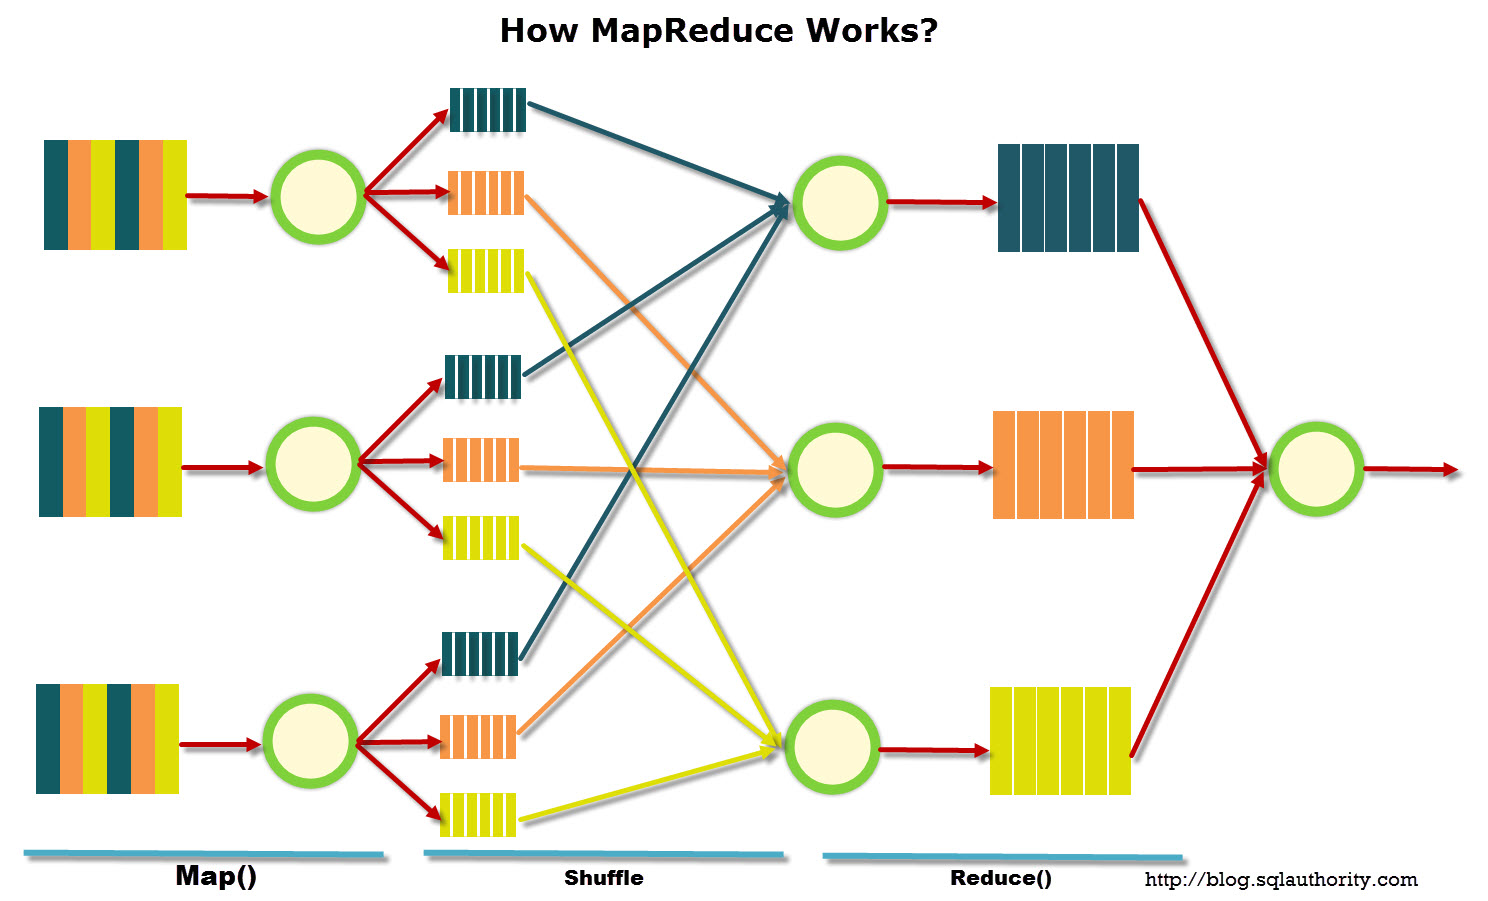
\includegraphics[width=\textwidth]{img/mapreduce.jpg}
\end{figure}
La Figura \ref{img:mapreduce} mostra il principio di funzionamento di un programma che applica Map Reduce. I dati vengono prelevati dai rispettivi dataset e suddivisi tra più macchine che effettuano il Map, in cui viene eseguito del codice per ogni singolo record. In questa fase vengono effettuati tutti i controlli descritti nel paragrafo \ref{sec:acquisizione}. In output si ottengono zero o più coppie chiave valore. Successivamente se sono presenti più unità di reduce i risultati vengono smistati tra di essi. Ogni unità di reduce si occupa di processare le coppie secondo la funzione di reduce, ed effettuano l'effettivo calcolo della statistica desiderata.



\subsection{Visualizzazione}\label{sec:visualizzazione}
La parte di visualizzazione è la parte più creativa ed interessante, parte principale in questa pubblicazione. Una volta effettuate le elaborazioni bisogna presentare i risultati, e si possono utilizzare tabelle o grafici. Con grafici si intendono diagrammi a barre, istogrammi, diagrammi a torte eccetera, quello che meglio può presentare ad un lettore il risultato elaborazioni. Una presentazione che permette di capire immediatamente il contenuto dei dati, utilizzando icone e simboli è sicuramente migliore di un'altra che presenta un grafico difficile da interpretare. Inoltre, è compito del data scientist decidere cosa mostrare, scegliendo cosa è interessante e cosa non lo è per raggiungere l'obbiettivo che si è preposto.

Gli strumenti a disposizione degli sviluppatori sono molteplici, da fogli elettronici come Excel o Calc di OpenOffice, programmi matematici come Matlab, fino alle librerie disponibili per i vari linguaggi di programmazione, sicuramente più complesse ma molto più potenti in fatto di personalizzazione. 

L'evoluzione del World Wide Web ha permesso la creazione di pagine interattive che supportano animazioni. Nel capitolo \ref{sec:d3} vedremo uno strumento web chiamato D3.js, il quale ci permette non solo di disegnare grafici in una pagina web, ma di gestire molti componenti grafici come rettangoli, cerchi, poligoni, \emph{mappe} e le loro animazioni.






\section{Pattern MVC}\label{sec:mvc}
\begin{quote}Un design pattern  descrive un problema che si ripete più e più volte nel nostro ambiente, descrive poi il nucleo della soluzione del problema, in modo tale che si possa usare la soluzione un milione di volte, senza mai applicarla alla stessa maniera\end{quote}

Questa definizione di \emph{Design Pattern} viene data da \cite[p. 2,3]{designpatterns}, l'autore cita a sua volta la definizione di pattern architettonici, mostrando la similitudine con quelli informatici.

Il pattern MVC si occupa di definire una struttura per il software che divide e rende autonome le parti di visualizzazione, elaborazione e memorizzazione dei dati (Fig. \ref{img:mvc}).

Questa struttura offre notevoli vantaggi in termini di pulizia, estensione e mantenimento del codice. Secondo \cite[p. 4]{designpatterns}
\begin{quote}
MVC consta di tre tipologie di oggetti. Il Model è l'oggetto dell'applicazione, il View è la sua rappresentazione a video, e il Controller definisce le reazioni dell'interfaccia grafica all'input dell'utente.
\end{quote}

\begin{figure}[ht!]
	\caption{Pattern MVC}
	\label{img:mvc}
	\centering
		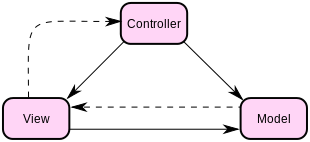
\includegraphics[width=\textwidth]{img/mvc1.png}
\end{figure}

Il programma sarà più pulito siccome in ogni sorgente sarà presente solamente il codice che si occupa di uno specifico compito. Non si presenterà quindi una situazione in cui nella stessa parte di codice oltre ad elaborare i dati ci dobbiamo preoccupare di formattarli per la presentazione su schermo, perché sarà compito della \emph{View}. L'aggiunta do nuove funzioni al software è molto semplice, per effettuare delle modifiche è spesso necessario aggiungere poche righe di codice in ogni parte del programma, senza il bisogno di stravolgerne la struttura. Il mantenimento del software risulta più semplice grazie alla suddivisione del codice in base al ruolo ed alla conseguente leggibilità.


\subsection{Model}
Il model, o \emph{modello} è la parte che si occupa della memorizzazione dei dati dell'applicazione, fornendo delle funzioni per salvare, leggere e modificare i dati dalla base dei dati. Le funzioni fornite sono l'\emph{interfaccia} attraverso cui il resto del programma può interagire con i dati dell'applicazione, non è possibile farlo direttamente sul database oppure in altri modi: rappresenta quindi uno strato al di sopra della base di dati, che ha il compito di fornire metodi ad alto livello per l'accesso ai dati, e di proteggere gli stessi da errori di programmazione comportati dall'accesso diretto.


\subsection{Controller}
Questa sezione si occupa di interfacciarsi con le altre due. Un controller in genere riceve le richieste dell'utente sotto forma di chiamate a funzioni e si occupa di eseguirle, preoccupandosi della validazione e della coerenza dei dati. Esso può essere un tramite tra \emph{View} e \emph{Model}, oppure operare solo con uno di loro:
\begin{itemize}
	\item Aggiunta di nuovi dati o modifica di dati esistenti
	
	Quando l'utente inserisce alcuni dati in un form e desidera che vengano memorizzati sul database, la View incapsula i dati inseriti in opportune strutture dati che verranno passate al controller, il quale effettuerà i controlli necessari per verificare che i dati non contengano errori, assicurarsi che non confliggano con quelli memorizzati, per poi inoltrare una richiesta di memorizzazione al Model, il quale eseguirà in modo del tutto trasparente al Controller l'operazione. Infine, il Controller invierà una conferma o l'errore alla View, in modo di informare l'utente su cosa ha fatto il sistema.
	\item Visualizzazione di dati
	
	In questo caso, la view invia una richiesta contenente le informazioni riguardanti a quali dati l'utente desidera visualizzare al Controller, quest'ultimo si occupa di verificare se l'utente è autorizzato ad accedere a quei dati restituendo errore nel caso in cui non sia autorizzato, oppure, se il Model supporta un sistema di gestione dei permessi ad utenti, inoltra la richiesta al model aggiungendo le informazioni sull'identità dell'utente.Il Model a questo punto provvederà a recuperare i dati e restituirli al Controller, effettuare alcune operazioni su di loro se necessario, per poi inviarle alla View.
\end{itemize}

I Controller sono quindi quelle parti del programma che si trovano tra l'interfaccia utente e la base di dati, che si occupano di coordinare le altre due componenti. Il loro compito è eseguire le richieste degli utenti, utilizzando le interfacce fornite da View e Model per portarle a termine, ma preoccupandosi anche dei controlli sui dati che transitano in essi.


\subsection{View}\label{sec:view}
La View è la parte che si occupa della \emph{visualizzazione} dei dati forniti dal controller. Essa utilizza nel sorgente dei \emph{placeholder} che verranno sostituiti a runtime dai dati.
Un esempio in campo web, potrebbe essere una semplice pagina che saluta il cliente e visualizza un elenco di prodotti in vendita:
\begin{lstlisting}
#View
Ciao {{nome}}!
Oggi in vendita abbiamo: {{for frutto in frutti}}
\end{lstlisting}
Le parti tra le doppie parentesi graffe\footnote{La sintassi di questo esempio è ispirata ad un \emph{Template Engine} chiamato Mustache (\url{http://mustache.github.io})} sono i placeholder, i quali possono contenere anche semplici istruzioni di ciclo o di confronto. Nel momento dell'esecuzione queste verranno sostituite con i dati indicati. Questo è necessario perché al momento della scrittura del programma le variabili "nome" e "frutti" non sono ancora stati calcolati!
Se i dati forniti dal controller sono questi:
\begin{lstlisting}
#Controller
nome="Andrea"
frutti=['pere', 'mele', 'arance']
\end{lstlisting}
Il risultato dell'esecuzione sarà quindi:
\begin{lstlisting}
Ciao Andrea!
Oggi in vendita abbiamo: pere mele arance
\end{lstlisting}

%%%%%%%SOFTWARE LATO SERVER%%%%%%%%
\section{Software lato server}\label{sec:server}
Come ogni sito web, per visualizzare una pagina sono necessari un browser internet ed un server che risponda alle richieste HTTP. Il browser si connetterà al server e quest'ultimo invierà la pagina, infine il browser si occuperà di visualizzarla interpretando il codice HTML ed eseguendo gli script lato client in esso contenuto.
\subsection{Turbogears}\label{sec:tg}
Turbo Gears 2 è un framework web scritto in \emph{Python}\footnote{Tutte le informazioni possono essere trovate sul sito ufficiale: \url{http://turbogears.org/}.}, esso permette la creazione di siti web in modo veloce e semplice applicando il pattern MVC. Fornisce la possibilità di scegliere quale Model utilizzare, fornendo una scelta fra database relazionali e non. Anche per gli altri componenti è possibile effettuare delle scelte, ma per lo sviluppo di questo progetto sono stati utilizzati quelli di default.
Turbo Gears può anche essere utilizzato come server web, siccome offre un modo molto semplice per avviarne uno.
TG analizza le richieste ricavando informazioni dall'url richiesto dal client. Un url come quello del listato \ref{ls:url} significa:
\begin{lstlisting}[label=ls:url,caption={Url per la richiesta di una pagina}]
http://www.tg2site.com/controller/function
\end{lstlisting}
		
\begin{description}
\item[http://www.tg2site.com] 
		
Nome dell'host
\item[controller]
		
Indica quale controller utilizzare. Questo può essere omesso, in tal caso verrà utilizzato il \emph{root controller}.
\item[function]
		
Indica quale funzione del controller si desidera richiamare.
\end{description}

In TG la \emph{view} è implementata utilizzando un linguaggio di markup simile all'html con l'aggiunta di \emph{marker} o \emph{segnaposto} che permettono di utilizzare un meccanismo simile a quello mostrato nel paragrafo \ref{sec:view}. Il modulo che si occupa della sostituzione del segnaposto con le informazioni si chiama Genshi.

Il \emph{model} invece è implementato utilizzando una libreria chiamata \emph{Ming}\footnote{\url{merciless.sourceforge.net/tour.html}}, la quale permette di definire delle classi di oggetti che avranno la caratteristica di rimanere sincronizzate con Mongo DB. Esso appartiene a quella classe di software che viene definito un \emph{ORM} (Object Relational Mapping). Tutti gli ORM forniscono la possibilità di associare una classe di un programma con una tabella del database, assicurando la \emph{consistenza} nei dati che si raggiunge con tecniche che permettono di creare un oggetto a partire da un record di un database, modificarlo e di occuparsi di memorizzare le modifiche, oppure creare direttamente un nuovo record. Il tutto avviene senza scrivere una riga del linguaggio di interrogazione del database, ci pensa ORM. 

A questo punto è lecito chiedersi perché la libertà offerta dalla natura \emph{NOSQL} di Mongo, ossia la mancanza della necessità di avere una struttura dati ben definita, viene eliminata utilizzando una libreria come Ming. Le ragioni dietro a questa scelta sono che questa proprietà di mongo è molto comoda nel momento dello sviluppo, durante il quale il database viene rigenerato più volte al giorno, ma diventa un problema quando si ha bisogno di una certa garanzia della tipologia di dati memorizzati in una certa \emph{collezione}\footnote{L'equivalente di una tabella, in Mongo, come verrà spiegato nel paragrafo \ref{sec:mongo}.}, inoltre l'utilizzo di un ORM aumenta la portabilità del progetto.

Ming è un'estensione adottata da TG per permettere l'utilizzo di Mongo, mentre SQLAlchemy è quello utilizzato per la controparte SQL.

La struttura tipo di un progetto TurboGears 2 è rappresentata nella figura \ref{fig:progetto}.
\begin{figure}[ht!]
	\caption{Struttura di un progetto TG2.}
	\label{fig:progetto}
	\centering
	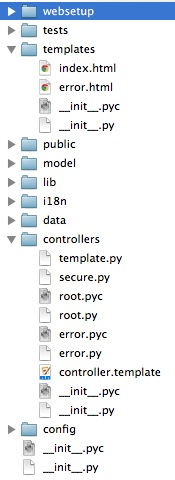
\includegraphics{img/tg2project.jpg}
\end{figure}

A seguire verranno descritte alcune delle cartelle più importanti.
\begin{description}
\item[model] contiene le classi necessarie a Ming per definire una struttura per i dati da salvare sul database.
\item[controllers] contiene i controller. \texttt{root.py} è il \emph{root controller}, \texttt{error.py}, creato da TG, si occupa della gestione degli errori.
\item[templates] contiene le pagine html del progetto.
\item[public] contiene tutte le risorse accessibili via web, come immagini, librerie JavaScript e fogli di stile.
\item[config e lib] contengono impostazioni e funzioni utili, utilizzate da TG e liberamente utilizzabili dal programmatore.
\end{description}

Il flusso di lavoro di TG potrebbe essere riassunto in:
\begin{enumerate}
\item Analizza l'url
\item Richiama l'opportuna funzione dell'opportuno controller
\item La funzione potrebbe interfacciarsi con il database, memorizzare o estrarre dati. 

In essa è sempre definito un \emph{decoratore} riconoscibile con la direttiva \texttt{expose}, con cui si indica alla View quale templare utilizzare. La funzione di un controller viene richiamata nel caso in cui TG riceve una richiesta del tipo \texttt{hostname/func/param1/param2/...}, i valori \texttt{param} sono i parametri della funzione, i dati da passare a Genshi devono essere memorizzati in un oggetto \texttt{dictionary} di python e restituiti dalla funzione. 
\item La view sostituisce i marker con le relative informazioni, infine genera la pagina
\item La pagina generata viene inviata al client che ha effettuato la richiesta.
\end{enumerate}

		
\subsection{Mongo DB}\label{sec:mongo}
Come spiegato nel capitolo \ref{sec:dbnonrel}, \emph{Mongo DB} è il DBMS utilizzato per il progetto, in cui vengono memorizzati i dati utilizzati dall'applicazione. Il sito ufficiale è \url{www.mongodb.org}, in cui oltre al programma si può trovare il manuale ed un tutorial interattivo. 

Mongo come linguaggio di interrogazione non utilizza SQL a causa della sua natura NOSQL, ma utilizza JavaScript. Importantissimi sono il concetto di \emph{documento} e \emph{collezione}, in quando a differenza del modello relazionale, in Mongo non esistono tabelle e relazioni, ma collezioni di documenti. Molto facilmente si potrebbe dire che una collezione è l'equivalente di una tabella nel modello relazionale ed un documento ad un record memorizzato in una tabella, ma le differenze si estendono alle chiavi primarie ed alle relazioni, siccome esse non esistono. Il tutto è molto semplificato rispetto al modello relazionale: per identificare univocamente ogni record si utilizza un campo \emph{id} come descritto più avanti, e per riferirsi a documenti di altre collezioni si memorizza un puntatore al documento stesso. Inoltre, ogni documento è un oggetto JavaScript, che può contenere come attributi liste e riferimenti ad altri oggetti. Nel database vengono memorizzati gli oggetti JavaScript tramite una funzione \texttt{save()}, ed è possibile estrarli utilizzando la funzione \texttt{find()}. Nel momento della creazione di un nuovo documento, Mongo aggiunge un campo \texttt{\_id} contenente un oggetto che rappresenta un identificativo univoco nella collezione, equivalente ad una chiave primaria di una tabella.
Per riferirsi ad una collezione si utilizza l'oggetto 
\texttt{database.collezione}
ossia, la collezione \texttt{collezione} è un attributo dell'oggetto \texttt{database}. Nell'oggetto collezione sono definiti i metodi per il salvataggio, la ricerca e l'eliminazione dei documenti prima citati. In particolare, per la funzione di ricerca, il parametro passato è un oggetto JavaScript contenente i parametri di ricerca, i quali valgono per i campi del documento: si può definire una ricerca per valori \emph{uguali}, \emph{maggiori}, \emph{minori} o \emph{diversi} da valori specificati. 

Il valore di ritorno è un iteratore, il quale è un oggetto che applica il pattern \emph{iterator}, il quale, brevemente, permette di definire un'interfaccia per scorrere una struttura dati, in modo da renderla virtualmente una lista di elementi accessibili sequenzialmente. In questo modo ad esempio, se si vuole percorrere un albero, una funzione \emph{successivo} di un iteratore che visita l'albero in \emph{profondità} restituirà la radice, il figlio della radice, poi il figlio del figlio della radice. Nel caso si voglia visitare l'albero in ampiezza, basterà istanziare un iteratore di quel tipo e si otterrà l'effetto desiderato, il tutto senza cambiare il codice della funzione che riceve gli elementi. Questo oggetto fornisce il metodo \texttt{next()}, che restituisce il documento successivo nella lista, ed offre la comodità di poter essere utilizzato in un ciclo \texttt{for} perché supportato nativamente da JavaScript.

\section{Librerie}\label{sec:librerie}
\subsection{d3.js}\label{sec:d3}
D3.js è una libreria JavaScript che offre strumenti molto potenti per la visualizzazione di dati, il sito ufficiale è raggiungibile alla pagina \url{http://d3js.org/}. La descrizione reperibile da esso, spiega che
\begin{quotation}
D3.js è un libreria JavaScript per la manipolazione di documenti basati sui dati. D3 fornisce gli strumenti per rappresentare i dati utilizzando HTML, SVG e CSS. D3 si focalizza sugli standard web offrendo tutta la potenza dei browser attuali senza essere dipendenti da un framework proprietario, combinando strumenti di visualizzazione con un approccio \emph{data-driven} per la manipolazione del DOM.
\end{quotation}
In pratica D3 permette di modificare il DOM di una pagina web in base ai dati collegati all'applicazione, utilizzando i tag \emph{SVG} di \emph{HTML}, acronimo di \emph{Scalable Vector Graphics}.
\emph{Protovis}, realizzato dal professor Jeff Heer, Vadim Ogievetsky e Mike Bostock della Stanford University, era una libreria JavaScript capace di creare grafica SVG a partire dai dati. Nel 2011 il suo sviluppo venne interrotto per spostare l'attenzione al suo successore, D3.js, creato dagli stessi tre sviluppatori ed in particolar modo da Mike Bostock, che oltre ad essere più performante si attiene ai più recenti standard web.\footnote{Fonte: \url{http://en.wikipedia.org/wiki/D3.js\#Context}}. 

Gli standard web sono una serie di regole e \emph{Best Practices} non proprietarie, che definiscono e descrivono gli aspetti del \emph{World Wide Web}. Uno degli enti che si occupa degli standard web è il World Wide Web Consortium o \emph{W3C}, che descrive gli elementi di HTML, CSS, JavaScript e non solo, fornendo spiegazioni esaustive di cono siano, come funzionano ed anche di come si usano. Il sito di W3C è \url{http://www.w3.org/}.

Gli strumenti che offre D3.js comprendono:
\begin{itemize}
\item Metodi di selezione

Il framework rispetta le \emph{W3C Selectors API}, uno standard alternativo alle API di manipolazione del DOM tradizionali. Con queste è possibile selezionare uno o più elementi nella pagina utilizzando diversi criteri, come il nome del \emph{tag}, l'\emph{id} o se un attributo è uguale ad un certo valore, ottenendo un array contenente tutti gli elementi conformi al criterio di selezione.

\item Binding dei dati

Dato un array in JavaScript, D3 permette di associarlo ad una funzione che si occuperà di eseguire del codice per ogni singolo elemento, con la possibilità di specificare cosa fare nel caso in cui questo array cambi, fornendo una funzione che viene richiamata quando degli elementi vengono aggiunti o eliminati. Quindi, dato un array contenente degli oggetti che rappresentano dei locali, lo si può associare ad un elemento Mappa che si occuperà di visualizzare in un canvas SVG un puntino per ogni locale nella giusta posizione su di una mappa.

\item Transizioni

Questa parte si occupa di fornire le primitive per animare le parti di una pagina. Definendo il tempo della transizione e lo stato finale di alcuni attributi, al momento dell'esecuzione del codice D3 si occupa di modificare in modo graduale gli attributi specificati fino da diventare come definiti nello stato finale. In questo modo si può modificare la posizione di un oggetto del DOM in modo che se si verifica un preciso evento, gradualmente si sposti verso l'esterno della pagina fino a scomparire, oppure per cambiarne il colore in modo graduale.
\end{itemize}

D3 permette lo sviluppo di grafici molto vari: diagrammi a torte, grafi e mappe interattive, il solo limite è la fantasia del programmatore. Sul sito principale si possono vedere molti esempi interessanti.
		
\subsection{Polymaps}\label{sec:polymaps}
Polymaps (\url{http://polymaps.org/}), scritta dallo stesso sviluppatore di D3.js Mike Bostock, è una libreria JavaScript che permette la creazione di mappe dinamiche ed è basata su D3. Offre numerose funzioni per la manipolazione di coordinate geospaziali, di mappe vettoriali o di mappe basate su immagini. Queste ultime possono essere ottenute tramite le funzioni fornite dalla libreria di siti come \emph{OpenStreetMaps} o \emph{Bing}.



